Nachdem das Verfahren für die Durchlichtauswertung Fehlstellen auf transparenten Objekten sichtbar machen konnte, stellt man sich die Frage, ob ähnliche Ergebnisse auch für nicht-transparente spiegelnde Objekte erzielt werden können.
Für diese Objekte wird das Verfahren mit der Spiegelbildauswertung angewandt.
Hierfür wählt man den Aufbau aus dem rechten Teilbild aus Abbildung \ref{tikz:abbAufbauFotos}.

\p
Für einen Vergleich der Spiegelbildauswertung zur Durchlichtauswertung für transparente Prüfobjekte wird das Brillenglas 1 (siehe linkes Teilbild aus Abbildung \ref{tikz:abbStreifenaufnahmen}) untersucht, da es ein polarisierendes Sonnenbrillenglas ist.
Das bedeutet, dass das Brillenglas das auftreffende Licht je nach Polarisation des Lichts deutlich stärker reflektiert.
Somit gelangt nahezu nur noch Licht mit einer speziellen Polarisation\footnote{
Die Polarisation beschreibt die Schwingungsrichtung der Lichtwellen.
Für den weiteren Verlauf sind die Details irrelevant, weshalb nicht konkreter darauf eingegangen werden muss.
} durch das Glas.
Diese Eigenschaft kann man für die Spiegelbildauswertung nutzen, um den Rückseitenreflex (vgl. Abschnitt \ref{sec:spiegelndeOberflaechen}) zu minimieren.
Die weiteren Objekte sind spiegelnde Keramikbruchstücke.
Die Prüfobjekte werden mittels eines Gelenkarms über dem Bildschirm positioniert und durch die Kamera aufgenommen (siehe Abbildung \ref{tikz:abbStreifenaufnahmenSpLichtstreuung}).

% Abbildung: Streifenaufnahmen
{
	\begin{figure}[H]
		\centering
		\begin{adjustbox}{width=\textwidth}
	\begin{tikzpicture}[every node/.style={inner sep=0,outer sep=0}]
		% Bilder
		\node [anchor=north west] (img1) at (0,0) {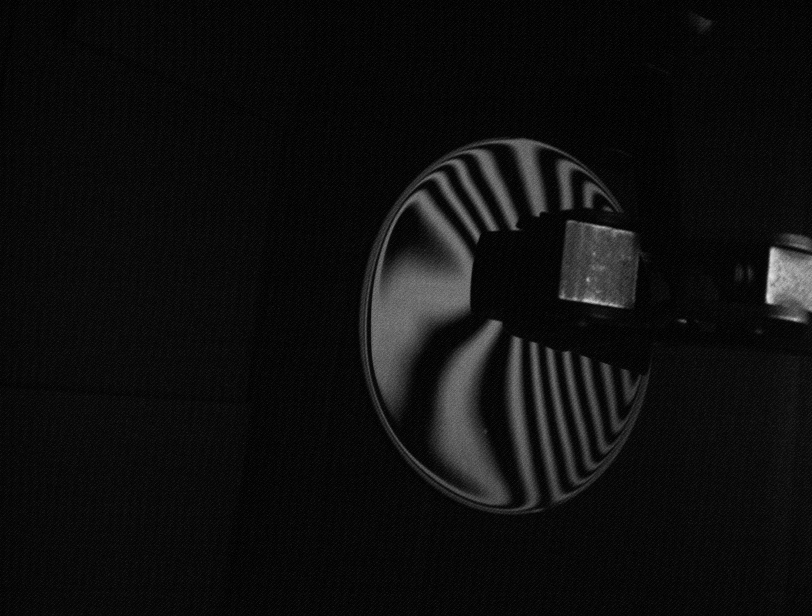
\includegraphics[width=.31\textwidth]{05_ergebnisse/ergSichtpruefungDurchLichtstreuung/spiegelbildAuswertungLichtstreuung/figures/brillenglas_1_beleuchtetImpuls}};
		\node [anchor=north west] (img2) at (0.345\textwidth,0) {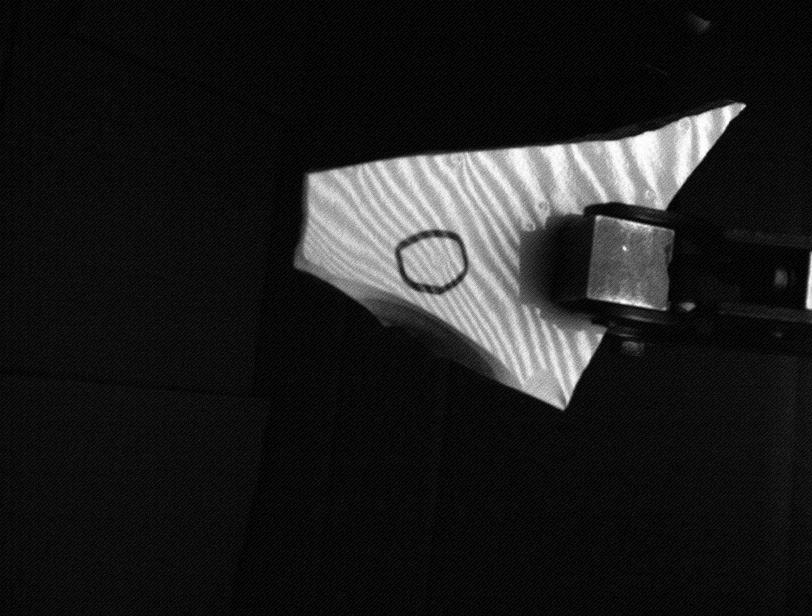
\includegraphics[width=.31\textwidth]{05_ergebnisse/ergSichtpruefungDurchLichtstreuung/spiegelbildAuswertungLichtstreuung/figures/keramikObjekt_1_beleuchtetImpuls}};
		\node [anchor=north west] (img3) at (0.69\textwidth,0) {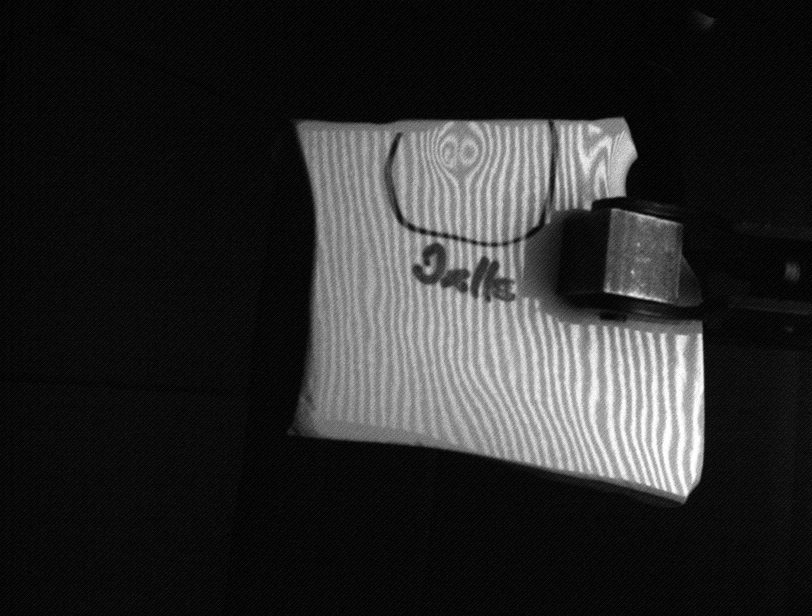
\includegraphics[width=.31\textwidth]{05_ergebnisse/ergSichtpruefungDurchLichtstreuung/spiegelbildAuswertungLichtstreuung/figures/keramikObjekt_2_beleuchtetImpuls}};
		
		% Captions
		\node [below=0.2cm of img1] (cap1) {Brillenglas 1};
		\node [below=0.2cm of img2] (cap2) {Keramikobjekt 1};
		\node [below=0.2cm of img3] (cap3) {Keramikobjekt 2};			
	\end{tikzpicture}
\end{adjustbox}
\caption[Aufnahmen der Streifenmuster bei der Spiegelbildauswertung]{Aufnahmen der Streifenmuster bei der Spiegelbildauswertung}
		\label{tikz:abbStreifenaufnahmenSpLichtstreuung}
	\end{figure}
}

\noindent
Durch Anwendung des Verfahrens \glqq Sichtprüfung durch Lichtstreuung\grqq ~erhält man für die drei Prüfobjekte folgende Bilder:

% Abbildung: Ergebnis der Sichtprüfung durch Lichtstreuung
{
	\begin{figure}[H]
		\centering
		\begin{adjustbox}{width=\textwidth}
	\begin{tikzpicture}[every node/.style={inner sep=0,outer sep=0}]
		% Bilder
		\node [anchor=north west] (img1) at (0,0) {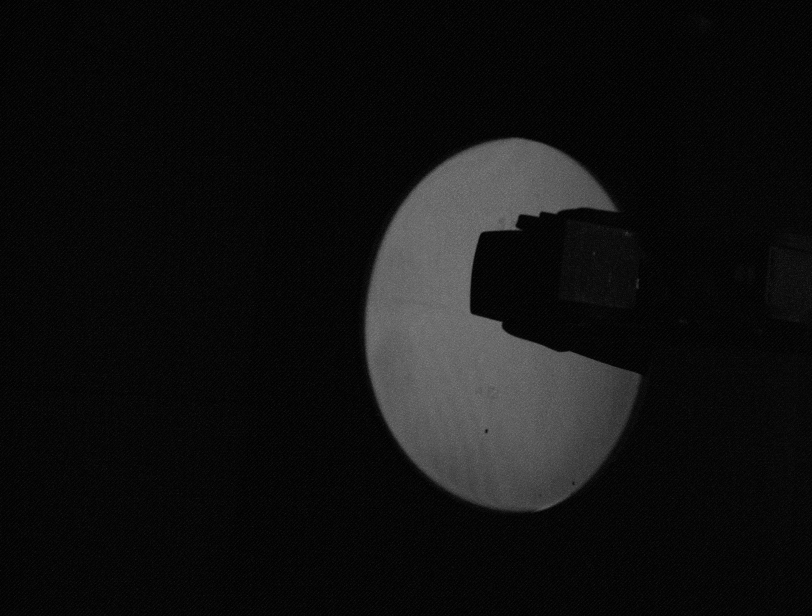
\includegraphics[width=.31\textwidth]{05_ergebnisse/ergSichtpruefungDurchLichtstreuung/spiegelbildAuswertungLichtstreuung/figures/brillenglas_1_combinePattern}};
		\node [anchor=north west] (img2) at (0.345\textwidth,0) {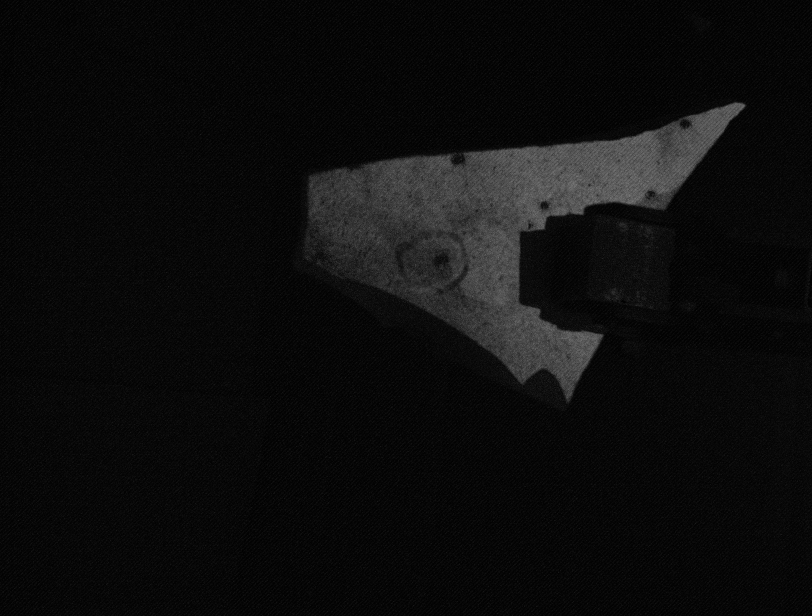
\includegraphics[width=.31\textwidth]{05_ergebnisse/ergSichtpruefungDurchLichtstreuung/spiegelbildAuswertungLichtstreuung/figures/keramikObjekt_1_combinePattern}};
		\node [anchor=north west] (img3) at (0.69\textwidth,0) {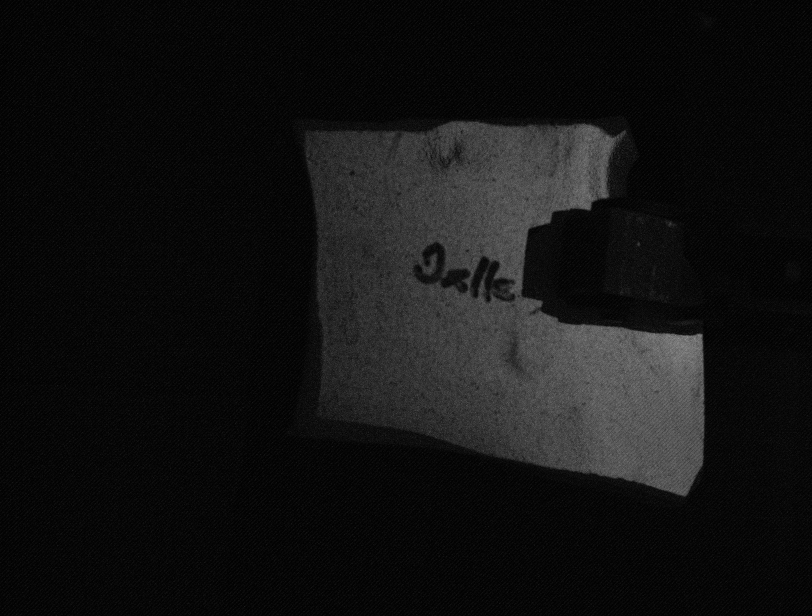
\includegraphics[width=.31\textwidth]{05_ergebnisse/ergSichtpruefungDurchLichtstreuung/spiegelbildAuswertungLichtstreuung/figures/keramikObjekt_2_combinePattern}};
		
		% Captions
		\node [below=0.2cm of img1] (cap1) {Brillenglas 1};
		\node [below=0.2cm of img2] (cap2) {Keramikobjekt 1};
		\node [below=0.2cm of img3] (cap3) {Keramikobjekt 2};		
	\end{tikzpicture}
\end{adjustbox}
\caption[Ergebnisbilder des Verfahrens \glqq Sichtprüfung durch Lichtstreuung\grqq ~bei der Spiegelbildauswertung]{Ergebnisbilder des Verfahrens \glqq Sichtprüfung durch Lichtstreuung\grqq ~bei der Spiegelbildauswertung}
		\label{tikz:abbCombinePatternPicturesSpLichtstreuung}
	\end{figure}
}

\noindent
Es wurde als Verknüpfungsmethode des Verfahrens die betragsmäßige Differenz gewählt, um die Bilder aus Abbildung \ref{tikz:abbCombinePatternPicturesSpLichtstreuung} zu erzeugen.
Wie auch im vorigen Abschnitt \ref{sub:durchlichtAuswertungLichtstreuung} ist der Grund dafür der höhere Kontrast zwischen den Prüfobjekten und dem Hintergrund.
In einem weiterem Schritt wurden die Bilder durch lokale Kontrastverbesserungen und geeignete Kennlinientransformationen nachbearbeitet, um die Fehlstellen besser zu erkennen:

% Abbildung: Nachbearbeitung der Ergebnisbilder
{
	\begin{figure}[H]
		\centering
		\begin{adjustbox}{width=\textwidth}
	\begin{tikzpicture}[every node/.style={inner sep=0,outer sep=0}]
		% Bilder
		\node [anchor=north west] (img1) at (0,0) {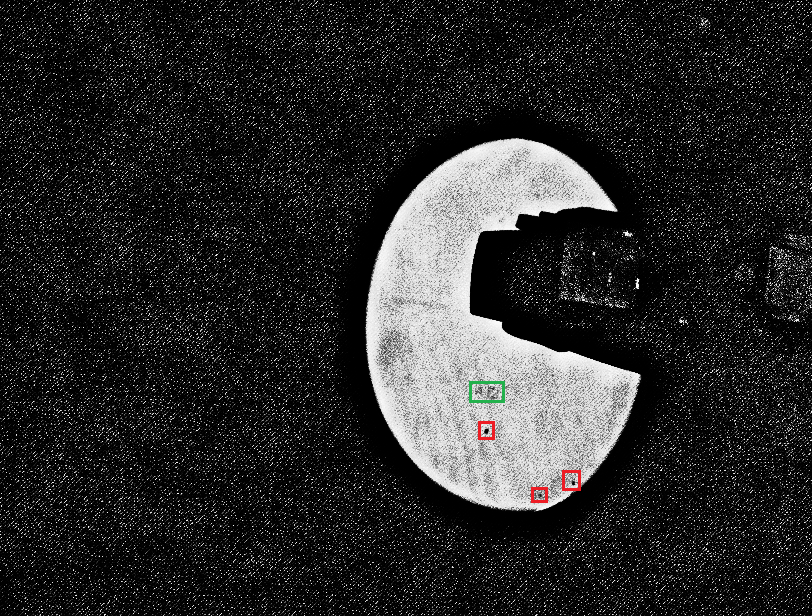
\includegraphics[width=.31\textwidth]{05_ergebnisse/ergSichtpruefungDurchLichtstreuung/spiegelbildAuswertungLichtstreuung/figures/brillenglas_1_verbessert}};
		\node [anchor=north west] (img2) at (0.345\textwidth,0) {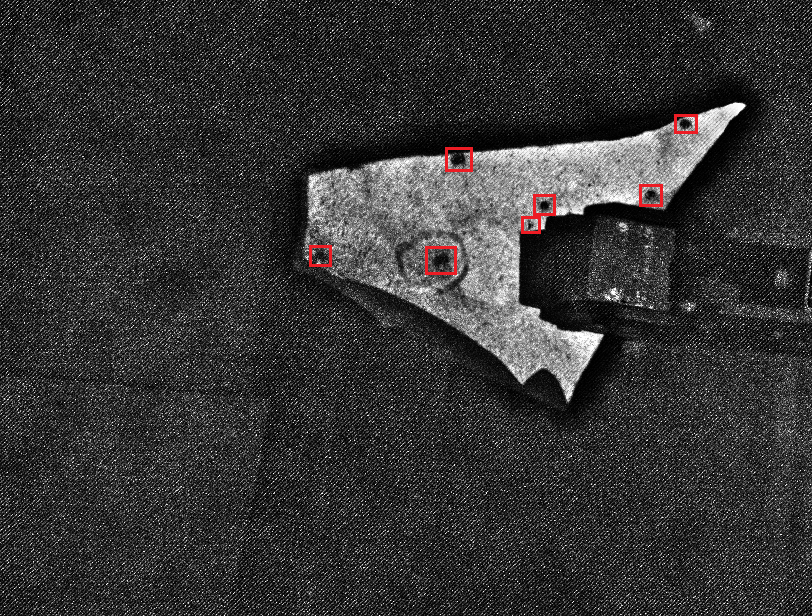
\includegraphics[width=.31\textwidth]{05_ergebnisse/ergSichtpruefungDurchLichtstreuung/spiegelbildAuswertungLichtstreuung/figures/keramikObjekt_1_verbessert}};
		\node [anchor=north west] (img3) at (0.69\textwidth,0) {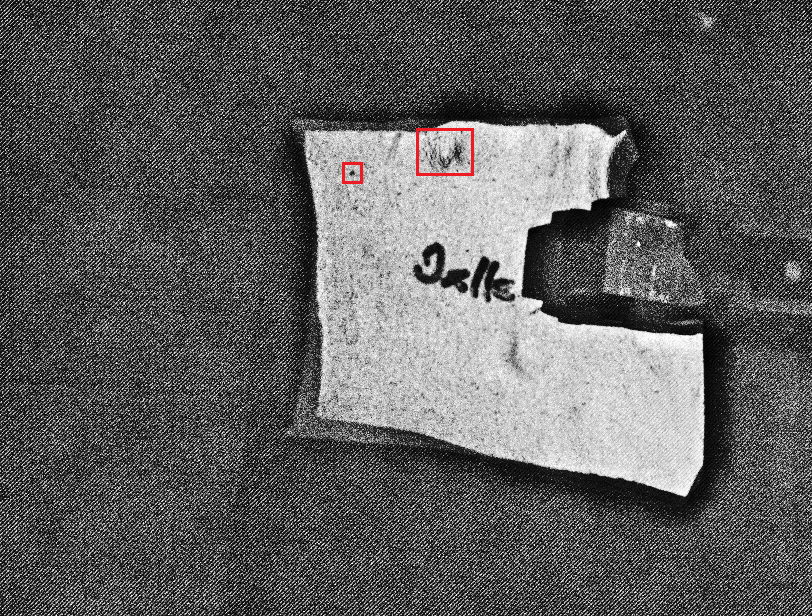
\includegraphics[width=.31\textwidth]{05_ergebnisse/ergSichtpruefungDurchLichtstreuung/spiegelbildAuswertungLichtstreuung/figures/keramikObjekt_2_verbessert}};
		
		% Captions
		\node [below=0.2cm of img1] (cap1) {Brillenglas 1};
		\node [below=0.2cm of img2] (cap2) {Keramikobjekt 1};
		\node [below=0.2cm of img3] (cap3) {Keramikobjekt 2};
	\end{tikzpicture}
\end{adjustbox}
\caption[Verbesserung der Ergebnisbilder]{Verbesserung der Ergebnisbilder. In Grün (bei Brillenglas 1): Gravur der Brillenglaskennzeichnung. In Rot: Kratzer, Pickel und ähnliche Be\-schä\-di\-gun\-gen der Oberfläche.}
		\label{tikz:abbNachbearbeitungSpLichtstreuung}
	\end{figure}
}

\noindent
In Abbildung \ref{tikz:abbNachbearbeitungSpLichtstreuung} sind die Fehlstellen in Rot markiert. 
Analog wie auch im vorherigen Abschnitt \ref{sub:durchlichtAuswertungLichtstreuung} erkennt man für Brillenglas 1 im grünen Rechteck eine Gravur des Markenzeichens auf der Oberfläche.
Für das Keramikobjekt 1 fallen einige dunkle Punkte im Objektbereich auf, welche durch sogenannte \glqq Pickel\grqq ~auf der Oberfläche entstehen.
Auf dem Keramikobjekt 2 befindet sich eine Delle, die im größeren roten Rechteck zu sehen ist.